\section{RLC Circuits}

\subsection{Circuits Review}

\subsubsection{Resistor}

\begin{itemize}
    \item $V = IR$
    \item $P = IV = I^2R = \frac{V^2}{R}$
\end{itemize}

\subsubsection{Capacitor}

\begin{itemize}
    \item $I = C \frac{dV}{dt}$
    \item $V = \frac{1}{C} \int I dt$
    \item $P = IV = CV \frac{dV}{dt} = \frac{V^2}{R}$
\end{itemize}

\subsubsection{Inductor}

\begin{itemize}
    \item $V = L \frac{dI}{dt}$
    \item $I = \frac{1}{L} \int V dt$
    \item $P = IV = LI \frac{dI}{dt} = \frac{I^2}{R}$
\end{itemize}

\subsection{RLC Circuits}

\subsubsection{Series RLC Circuit}

\begin{wrapfigure}{r}{0.5\textwidth}
    \centering
    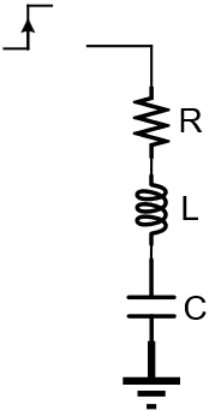
\includegraphics[scale=0.5]{images/RLC.png}
    \caption{RLC Circuit}
\end{wrapfigure}

Wires have resistance, inductance and capacitance. Thus the circuit is not ideal. 

For a change of voltage to propagate through the wire, it takes time.

\subsubsection{Rise/Fall Time}

Rise time is the time it takes for the voltage to rise from 10\% to 90\% of the final value.

Fall time is the time it takes for the voltage to fall from 90\% to 10\% of the final value.

If there is no inductance, then the time of fall $t_f = RC \times \ln(9) = 2.2RC$.

Let $\tau = RC$, then $t_f = 2.2\tau$. If $\tau$ is too large, the signal will converge given a fluctating input since it never reaches the final value before the next fluctuation.